\documentclass[a4paper]{article}

\usepackage[english]{babel}
\usepackage[utf8]{inputenc}
\usepackage[T1]{fontenc}       %makes text copy-and-pastable
\usepackage{wrapfig}           %for figures
\usepackage{graphicx}          %for images
\usepackage{booktabs}          % good tables package
\usepackage{array}             %for spacing tables
\usepackage{multirow}          %for multirow tables
\usepackage{caption}           %for the captionof command
\usepackage{amsmath}           %for any moderately complex math
\usepackage{placeins}          %allows us to use \FloatBarrier
\usepackage{caption}           %to use minipage for inserting figures
\usepackage{float}             %for H figure and table placements Here.
\usepackage{comment}          %for bulk comments
\usepackage[colorinlistoftodos]{todonotes}%to do notes
\usepackage[parfill]{parskip}  %To use blank lines instead of indentation to separate paragraphs
\usepackage{ifthen}            %ifthenelse command
\usepackage[margin=3cm]{geometry} %Change margin size
\usepackage{titling}           %for spacing the title
\usepackage{blindtext}         %for spacing the title
    \setlength{\droptitle}{-4em}     % For spacing the title
    \addtolength{\droptitle}{-4pt}   % For spacing the title
%\usepackage[super]{nth}        %write 1st,2nd,3rd with \nth{1},\nth{2}, \nth{3}
%\usepackage{ifdraft}
\usepackage{units}
\usepackage{subcaption} % for subfigures
\captionsetup{width=0.8\textwidth}


\usepackage{tikz}
\usepackage{calc}
% \usepackage{pgfgantt}             %For gantt charts
\usepackage{pgffor}
\usepackage[american]{circuitikz}
\usepackage{ifthen}
\usepackage{pgfplots}
\pgfplotsset{compat=1.13}
\usetikzlibrary{decorations.pathreplacing}

\usepackage{varioref}

\usepackage[hidelinks,%clickable cross references and URLs
            pdftex,%pdf meta data
            pdfauthor={Matthew Davis},%pdf meta data
            pdftitle={ELEC4614 2013 Solutions},%pdf meta data
            %pdfsubject={\@title},%pdf meta data
            pdfkeywords={UNSW, ELSOC, ELEC4614, Power, Electronics, Past, Paper, Exam, Solutions, supp, supplementary}]{hyperref}

\usepackage[nameinlink, capitalise, noabbrev]{cleveref}

\title{ELEC4614 2013 S1 Supplementary Exam Solutions}
\author{Matthew Davis \\ \href{mailto:vicepresident@elsoc.net}{vicepresident@elsoc.net}}

\renewcommand\thesection{Question \arabic{section}}
\renewcommand\thesubsection{(\alph{subsection})}
\renewcommand\thesubsubsection{\roman{subsubsection})}

\usepackage{tocloft}
\usepackage{chngcntr}
\setlength{\cftsecnumwidth}{6em}
%\setlength{\cftsubsecnumwidth}{3.25em}
\setlength{\cftsubsubsecnumwidth}{4em}




\begin{document}

\maketitle

\begin{abstract}
    These are the unofficial solutions to the 2013 Semester 1 Power Electronics exam.
    There are two different 2013 exams. 
    These solutions abre for the one where question 1a has an inductor, which is the supplementary exam.
    The other exam is available on the library website.
    This is just the first draft. I don't guarantee than the solutions here are correct. If you spot a mistake, please let me know. I've put orange boxes throughout to indicate where I'm unsure.
    More solutions, papers and notes can be found at \href{www.elsoc.net}{elsoc.net}.
    Please note that for this particular exam, you only needed to solve 4 out of 6 possible questions.
\end{abstract}

%\listoftodos

\tableofcontents

\section{Half-Wave Rectifiers}

\subsection{}\label{sec:1a}

Assuming that the voltage source has amplitude $V_s$, not $\sqrt{2}V_s$.

\begin{center}


% \begin{figure}[htbp]
%     \centering
%     \begin{subfigure}[b]{\linewidth}
%       \centering
       
\begin{tikzpicture}%[node distance = 2 cm, scale=1]


\begin{axis}[domain=0:400, 
             axis x line=middle, 
             axis y line=left, 
             xtick={180,360}, 
             xticklabels={$\pi$,$2\pi$},
             ytick={-1,1},
             yticklabels={$-V_s$,$V_s$},
             x axis line style={->},
             xlabel={$\omega{}t$},
             xlabel style={align=right}, 
             y axis line style={->},
             width=0.8\textwidth,
             height=6cm,
             %width=\uncontrolledRectifierGraphWidth,
             ymax=1.2,
             ymin=-1.2,
             ] 
    \addplot[dashed, red, domain=180:360] {sin(x)}; 
    \addplot[blue, samples=360] {truncSin(x,0,180)};  
    \legend{$v_S$, $v_L$}
\end{axis}


\end{tikzpicture}
    %   \caption{Supply voltage ($v_S$) and load voltage ($v_L$)}
    %   \label{1a fig:uncontrolled voltage graph}
    % \end{subfigure}
    \vspace{2cm} \\
    % \begin{subfigure}[b]{\linewidth}
    %   \centering
       
\begin{tikzpicture}%[node distance = 2 cm, scale=1]


\begin{axis}[domain=0:400, 
             axis x line=middle, 
             axis y line=left, 
             xtick={180,360}, 
             xticklabels={$\pi$,$2\pi$},
             ytick={0,1},
             yticklabels={{\color{white}$-V_s$},$\frac{V_s}{R}$},
             x axis line style={->},
             xlabel={$\omega{}t$},
             xlabel style={align=right}, 
             y axis line style={->},
             width=0.8\textwidth,
             height=6cm,
             %width=\uncontrolledRectifierGraphWidth,
             ymax=1.2,
             %ymin=0,
             ] 
    \addplot[green, samples=360] {truncSin(x,0,180)}; 
    \legend{$i_L$}
\end{axis}


\end{tikzpicture}
%       \caption{Load current ($i_L$)}
%       \label{1a fig:uncontrolled current graph}
%     \end{subfigure}
%     \caption{Current and voltage waveforms for Q1a}
%     \label{1a fig:uncontrolled rectifier graphs}
% \end{figure}
\end{center}

\begin{align*}
V_{AV} & = \frac{1}{2\pi} \int_0^{2\pi} V_L(\omega{}t) d \omega t \\
       & = \frac{1}{2\pi} \int_0^{\pi} V_s\sin(\omega{}t) d \omega t \\
       & = \frac{V_s}{2\pi} \left[ -\cos(\omega{}t) d \right]_0^{\pi} \\   
       & = \frac{V_s}{2\pi} \left[ --1 --1 \right] \\   
       & = \frac{V_s}{\pi} \\
\intertext{\todo[inline]{Hmm. Is that right?}}
I_{AV} & = \frac{V_{AV}}{R} \\
       & = \frac{V_s}{R\pi}
\end{align*}


\subsection{}

\subsection{}

\subsection{}

\section{Fully Controlled Rectifier}

\subsection{}

\subsection{}

\xdef\myAlpha{30}
\pgfmathparse{\myAlpha + 180}
\xdef\mySecondAlpha{\pgfmathresult}


\begin{center}


\begin{tikzpicture}
\begin{axis}[domain=0:400, 
             axis x line=middle, 
             axis y line=left, 
             xtick={\myAlpha,180,\mySecondAlpha,360}, 
             xticklabels={$\alpha$,$\pi$,$\pi+\alpha$,$2\pi$},
             ytick={0},
             yticklabels={0},
             x axis line style={->},
             xlabel={$\omega{}t$},
             xlabel style={align=right}, 
             y axis line style={->},
             width=0.8\textwidth,
             height=6cm,
             %width=\uncontrolledRectifierGraphWidth,
             ymax=1.2,
             ymin=-1.2,
             ] 
    \addplot[blue] coordinates
    {
    (0,0)
    (\myAlpha,0)
    (\myAlpha,1)
    (180,1)
    (180,0)
    (180+\myAlpha,0)
    (180+\myAlpha,-1)
    (360,-1)
    (360,0)
    (360+\myAlpha,0)
    (360+\myAlpha,1)
    (400,1)
    }
    ; 
    \legend{$v_S$, $i_{ac}$}
\end{axis}
\end{tikzpicture}


\begin{tikzpicture}
\begin{axis}[domain=0:400, 
             axis x line=middle, 
             axis y line=left, 
             xtick={\myAlpha,180,\mySecondAlpha,360}, 
             xticklabels={$\alpha$,$\pi$,$\pi+\alpha$,$2\pi$},
             ytick={0},
             yticklabels={0},
             x axis line style={->},
             xlabel={$\omega{}t$},
             xlabel style={align=right}, 
             y axis line style={->},
             width=0.8\textwidth,
             height=6cm,
             %width=\uncontrolledRectifierGraphWidth,
             ymax=1.2,
             %ymin=0,
             ] 
    \addplot[red, samples=400] {
    and(1,mod(x,180)>\myAlpha)*
    sin(mod(x,180))}; 
    \legend{$v_S$, $i_{ac}$}
\end{axis}
\end{tikzpicture}
\end{center}
\subsection{}

\subsection{}

\section{H Bridge Inverter}

\begin{center}

% \begin{figure}[htbp]
%     \centering
    \includegraphics[page=6,
                 clip, 
                 trim=4.5cm 15.5cm 5cm 7cm]{3/figures/fullBridge.pdf}
    % \caption{H bridge inverter}
%     \label{fig:full bridge}
% \end{figure}
\end{center}

\subsection{}

The voltage applied to the load is just a square wave, with an amplitude of $V_d=\unit[200]{V}$.
The RMS value of a square wave (no dc offset) is just the height.

$$
V_{L_{rms}} = V_d = \unit[200]{V}
$$

\todo[inline]{2 marks for that? Am I missing something? Do they want us to actually do the integral?}
\subsection{}

\begin{align*}
a_1 & = \frac{4V_d}{\pi} = \frac{4\times 200}{\pi} = 254.64 \\
a_3 & = \frac{4V_d}{3\pi} = \frac{4\times 200}{3\pi} = 84.88 \\
a_5 & = \frac{4V_d}{5\pi} = \frac{4\times 200}{5\pi} = 50.92 \\
a_7 & = \frac{4V_d}{7\pi} = \frac{4\times 200}{7\pi} = 36.38 \\
a_9 & = \frac{4V_d}{9\pi} = \frac{4\times 200}{9\pi} = 28.29 \\
\end{align*}

\subsection{}

\begin{center}



\begin{tikzpicture}
\begin{axis}[domain=0:400, 
             axis x line=middle, 
             axis y line=left, 
             xtick={180,360}, 
             xticklabels={%\unit[1.678]{ms},
                          \unit[10]{ms},
                          \unit[20]{ms},
                          },
             ytick={-0.8,0.8},
             yticklabels={$-V_d$,$V_d$},
             x axis line style={->},
             xlabel={$\omega{}t$},
             xlabel style={align=right}, 
             y axis line style={->},
             width=0.8\textwidth,
             height=6cm,
             %width=\uncontrolledRectifierGraphWidth,
             ymax=1.2,
             ymin=-1.2,
             ] 
    \addplot[red, samples=1000] {+0.8-1.6*and(1,mod(x,360)>180)}; 
    \legend{$v_S$}
\end{axis}
\end{tikzpicture}


\xdef\Resistance{2}
\xdef\Inductance{0.005}
\xdef\Period{0.02}
\xdef\IO{-96.4}
\xdef\Vd{200}

\begin{tikzpicture}
\begin{axis}[domain=0:400, 
             axis x line=middle, 
             axis y line=left, 
             xtick={30.366,180,360}, 
             xticklabels={\unit[1.678]{ms},
                          \unit[10]{ms},
                          \unit[20]{ms},
                          },
             ytick={-96.4,96.4},
             yticklabels={%$-\frac{V_d}{R}{=}-100$,
                          $I_0{=}-96.4$,
                          $-I_0{=}96.4$,
                          %$\frac{V_d}{R}{=}100$},
                          },
             x axis line style={->},
             xlabel={$t$},
             xlabel style={align=right}, 
             y axis line style={->},
             width=0.8\textwidth,
             height=6cm,
             %width=\uncontrolledRectifierGraphWidth,
             ymax=110,
             ymin=-110,
             legend style={at={(axis cs:380,70),anchor=south west}}
             ] 
    \addplot[blue, samples=1000] {
    (and(1,mod(x,360)<180)-0.5)*2*
    (
       (\Vd/\Resistance) + (\IO-\Vd/\Resistance) *    exp(-\Resistance*mod(x,180)*\Period/(\Inductance*360))
    )
    }; 
    \addplot[blue, dotted, samples=1000, domain=180:400, ->] {
       (\Vd/\Resistance) + (\IO-\Vd/\Resistance) *    exp(-\Resistance*x*\Period/(\Inductance*360))
    };% 
    \node[right] at (400,100) {to $\frac{V_d}{R}{=}\unit[100]{A}$}; 
    \addplot[blue, dotted, samples=1000, domain=360:400, ->] {(-1)*(
       (\Vd/\Resistance) + (\IO-\Vd/\Resistance) *    exp(-\Resistance*(x-180)*\Period/(\Inductance*360))
       )
    };
    \node[right] at (400,-100) {to $\frac{-V_d}{R}{=}\unit[-100]{A}$}; 
    \legend{$i_L$}
\end{axis}
\end{tikzpicture}

%
\xdef\Resistance{2}
\xdef\Inductance{0.005}
\xdef\Period{0.02}
\xdef\IO{-96.4}
\xdef\Vd{200}


\begin{center}
\begin{tikzpicture}
\begin{axis}[domain=0:400, 
             axis x line=middle, 
             axis y line=left, 
             xtick={30.366,180,360}, 
             xticklabels={\unit[1.678]{ms},
                          \unit[10]{ms},
                          \unit[20]{ms},
                          },
             ytick={-96.4,96.4},
             yticklabels={%$-\frac{V_d}{R}{=}-100$,
                          $I_0{=}-96.4$,
                          $-I_0{=}96.4$,
                          %$\frac{V_d}{R}{=}100$},
                          },
             x axis line style={->},
             xlabel={$t$},
             xlabel style={align=right}, 
             y axis line style={->},
             width=0.8\textwidth,
             height=6cm,
             %width=\uncontrolledRectifierGraphWidth,
             ymax=110,
             ymin=-110,
             legend style={at={(axis cs:380,70),anchor=south west}}
             ] 
    \addplot[blue, samples=1000] {
    (and(1,mod(x,360)<180)-0.5)*2*
    (
       (\Vd/\Resistance) + (\IO-\Vd/\Resistance) *    exp(-\Resistance*mod(x,180)*\Period/(\Inductance*360))
    )
    }; 
    \addplot[blue, dotted, samples=1000, domain=180:400, ->] {
       (\Vd/\Resistance) + (\IO-\Vd/\Resistance) *    exp(-\Resistance*x*\Period/(\Inductance*360))
    };% 
    \node[right] at (400,100) {to $\frac{V_d}{R}{=}\unit[100]{A}$}; 
    \addplot[blue, dotted, samples=1000, domain=360:400, ->] {(-1)*(
       (\Vd/\Resistance) + (\IO-\Vd/\Resistance) *    exp(-\Resistance*(x-180)*\Period/(\Inductance*360))
       )
    };
    \node[right] at (400,-100) {to $\frac{-V_d}{R}{=}\unit[-100]{A}$}; 
    \legend{$i_L$}
\end{axis}
\end{tikzpicture}
\end{center}

\end{center}


\begin{align*}
I_0 & = -\frac{200}{2} \times \frac{1-e^{-\frac{2*0.01}{0.005}}}{1+e^{-\frac{2*0.01}{0.005}}} \\
    & = \unit[-96.4]{A} \\
0   & = i(t) \\
    & = \frac{V_d}{R} + \left( I_0 - \frac{V_d}{R}\right) e^{-\frac{R}{L}t} \\
\frac{V_d}{R} & = \left(\frac{V_d}{R} - I_0\right) e^{-\frac{R}{L} t} \\
\frac{\frac{V_d}{R}}{\frac{V_d}{R}-I_0} & = e^{-\frac{R}{L}t} \\
-\frac{R}{L}t = \ln\left(\frac{V_d}{V_d - I_0 R}\right) \\
t_0 & = -\frac{L}{R} \ln \left( \frac{V_d}{V_d-I_0R}\right) \\
    & = \frac{L}{R} \ln \left( \frac{V_d-I_0R}{V_d}\right) \\
    & = \frac{0.005}{2} \ln \left( \frac{200--96.4\times 2}{200}\right) \\
    & = \unit[1.687]{ms}
\end{align*}

(Sanity check: this is less than \unit[10]{ms}.)


\subsection{}

\todo[inline]{How do you use the result from part C? What result are they refering to? Do they mean the formulas they gave you in the question?}

Let $T=\unit[20]{ms}$ be the period.

\begin{align*}
I_{SW_{AVE}} & = \frac{1}{T} \int_0^{\frac{T}{2}} \frac{V_d}{R} + \left(I_0-\frac{V_d}{R}\right) e^{-\frac{R}{L}t} dt \\
& = \frac{1}{T} \left[\frac{V_d}{R}t + \left(I_0-\frac{V_d}{R}\right)\left(-\frac{L}{R}\right) e^{-\frac{R}{L}t} \right]_0^{\frac{T}{2}}\\
& = \frac{1}{T} \left[\frac{V_dT}{2R} + \left(I_0-\frac{V_d}{R}\right)\left(-\frac{L}{R}\right) \left(e^{-\frac{RT}{2L}}-1\right) \right]\\
& = \frac{1}{0.02} \left[\frac{200\times 0.02}{2\times 2} + \left(-96.4-\frac{200}{2}\right)\left(-\frac{0.005}{2}\right) \left(e^{-\frac{2\times0.02}{2\times 0.005}}-1\right) \right]\\
& = \unit[25.90]{A}
\end{align*}
\subsection{}


\xdef\Resistance{2}
\xdef\Inductance{0.005}
\xdef\Period{0.02}
\xdef\IO{-96.4}
\xdef\Vd{200}


\begin{center}
\begin{tikzpicture}
\begin{axis}[domain=0:400, 
             axis x line=middle, 
             axis y line=left, 
             xtick={30.366,180,360}, 
             xticklabels={\unit[1.678]{ms},
                          \unit[10]{ms},
                          \unit[20]{ms},
                          },
             ytick={-96.4,96.4},
             yticklabels={%$-\frac{V_d}{R}{=}-100$,
                          $I_0{=}-96.4$,
                          $-I_0{=}96.4$,
                          %$\frac{V_d}{R}{=}100$},
                          },
             x axis line style={->},
             xlabel={$t$},
             xlabel style={align=right}, 
             y axis line style={->},
             width=0.8\textwidth,
             height=6cm,
             %width=\uncontrolledRectifierGraphWidth,
             ymax=110,
             ymin=-110,
             legend style={at={(axis cs:380,70),anchor=south west}}
             ] 
    \addplot[blue, samples=1000] {
    (
       (\Vd/\Resistance) + (\IO-\Vd/\Resistance) *    exp(-\Resistance*mod(x,180)*\Period/(\Inductance*360))
    )
    }; 
    \addplot[blue, dotted, samples=1000, domain=180:400, ->] {
       (\Vd/\Resistance) + (\IO-\Vd/\Resistance) *    exp(-\Resistance*x*\Period/(\Inductance*360))
    };% 
    \node[right] at (400,100) {to $\frac{V_d}{R}{=}\unit[100]{A}$}; 
    \addplot[blue, dotted, samples=1000, domain=360:400, ->] {(1)*(
       (\Vd/\Resistance) + (\IO-\Vd/\Resistance) *    exp(-\Resistance*(x-180)*\Period/(\Inductance*360))
       )
    };
    \legend{$I_d$}
\end{axis}
\end{tikzpicture}
\end{center}
\subsection{}

\begin{align*}
a_n & = \frac{2}{\pi} \int_0^\pi V_L(t) \sin(n\omega{}t) d\omega t \\
    & = \frac{2}{\pi} \int_{\frac{\delta}{2}}^{\pi-\frac{\delta}{2}} V_d \sin(n\omega{}t) d\omega t \\
    & = \frac{2V_d}{n\pi} \left[- \cos(n\omega{}t) \right]_{\frac{\delta}{2}}^{\pi-\frac{\delta}{2}} \\
    & = \frac{2V_d}{n\pi} \left[\cos(\frac{n\delta}{2})-\cos\left(n\left(\pi-\frac{\delta}{2}\right)\right) \right] \\
    & = \frac{2V_d}{n\pi} \times 2\cos\left(\frac{n\delta}{2}\right) \\
    & = \frac{4V_d}{n\pi}\cos\left(\frac{n\pi}{3}\right)
\end{align*}

For $n=3$, $\cos\left(\frac{n\pi}{3}\right)=0$, so $a_3=0$.
i.e. The third harmonic dissappears.
 
\begin{align*}
a_1 & = \frac{4V_d}{\pi}\cos\left(\frac{\pi}{3}\right) \\
    & = \frac{4\times 200}{\pi}\times\frac{1}{2} \\
    & = \unit[127.3]{V}
\end{align*}
\renewcommand\thesubsection{(\roman{subsection})}
\section{3 Phase Inverter}

\subsection{}
\clearpage
\subsection{}

\pgfmathdeclarefunction{lineLineV}{1}{%
  \pgfmathparse{%
    and(1,mod(#1,180) < 120) * 
    (2 * and(1,mod(#1+360*3,360) < 180) - 1)
  }%
}

\newcommand\lineLineVPlot[2]{

\begin{tikzpicture}[]
\begin{axis}[standard,
             xlabel={$\omega t$},
             ylabel={$V_{#2}$},
             xtick={60,120,180,240,300,360,420}, 
             xticklabels={$\frac{\pi}{3}$,
                          $\frac{2\pi}{3}$,
                          $\pi$,
                          $\frac{4\pi}{3}$,
                          $\frac{5\pi}{3}$,
                          $2\pi$,
                          $\frac{7\pi}{3}$
                          },
             ytick={-1,1},
             yticklabels={$-V_{dc}$,$V_{dc}$},
             domain=0:430,
             width=0.8\textwidth,
             height=5cm,
             ymax=1.2,
             ymin=-1.2,
             ] 
    \addplot[blue, samples=430] {lineLineV(x-#1)}; 
    % \legend{$T_{#1}$}
\end{axis}
\end{tikzpicture}
}

\begin{centering}
   \foreach \wt/\l in {0/{AB},
                       120/{BC},
                       240/{CA}
                       }{
   
      \lineLineVPlot{\wt}{\l}
      
   }
\end{centering}
\subsection{}
\subsection{}
\subsection{}

The magnitude of the line-neutral voltage components are $\frac{1}{\sqrt{3}}$ of the line-line voltage components.
The current components are $\frac{1}{R}$ times the line-neutral voltage components. (Since there is no inductor in the load.)

\begin{align*}
i_n & = \frac{V_{ll}}{\sqrt{3}R} \\
i_1 & \frac{116.95}{\sqrt{3} \times 10} = 6.752 \\
i_5 & \frac{23.39}{\sqrt{3} \times 10} = 1.35 \\
i_7 & \frac{16.71}{\sqrt{3} \times 10} = 0.96 \\
i_{11} & \frac{10.63}{\sqrt{3} \times 10} = 0.61 \\
i_{13} & \frac{9.00}{\sqrt{3} \times 10} = 0.52 \\
\end{align*}
\subsection{}

\todo[inline]{5 marks for plotting a DC curve? That's too much. Did I get the answer wrong?}

The supply always sees a load of $R + (R\Vert R)=1.5R$. Therefore the current is always

\begin{align*}
i_{dc} & = \frac{V_{dc}}{1.5R} \\
       & = \frac{300}{1.5 \times 10} \\
       & = \unit[2]{A}
\end{align*}

\begin{center}
    \begin{tikzpicture}[]
\begin{axis}[standard,
             xlabel={$\omega t$},
             ylabel={$I_{dc}$},
             xtick={60,120,180,240,300,360,420}, 
             xticklabels={$\frac{\pi}{3}$,
                          $\frac{2\pi}{3}$,
                          $\pi$,
                          $\frac{4\pi}{3}$,
                          $\frac{5\pi}{3}$,
                          $2\pi$,
                          $\frac{7\pi}{3}$
                          },
             ytick={2},
            %  yticklabels={},
             domain=0:430,
             width=0.8\textwidth,
             height=5cm,
             ymax=2.4,
             ymin=0,
             ] 
    \addplot[blue] {2}
    ; 
\end{axis}
\end{tikzpicture}
\end{center}
\renewcommand\thesubsection{(\alph{subsection})}
\section{Isolated DC-DC Converters}

\subsection{}

\subsection{}

\subsection{}

\section{Losses and Switching}

\subsection{}


\subsection{}

\subsection{}

\subsection{}

\subsection{}

\subsection{}

Total power is

\begin{align*}
P & = P_D + P_T \\
  & = 13.5 + 66\\
  & = \unit[79.5]{W}
\end{align*}


\begin{center}

\begin{circuitikz}%[node distance = 2 cm, scale=1]
\xdef\topy{3}
\xdef\midx{4}
\xdef\rightx{8}

\draw (0,0) node[ground] {}
      to[current source, l={\unit[7.7]{W}}, -*] (0,\topy)
      node[above] {$70^\circ$}
      to[R, l={\unit[0.2]{$^\circ$K/W}}] (\midx,\topy)
      to[R, l=$x$] (\rightx,\topy)
      
      (\rightx,0) node[ground] {}
      to[battery1, l={$40^\circ$}]
      (\rightx,\topy)
      ;
\end{circuitikz}
\end{center}

\begin{align*}
90 & = 45 + 79.5 x \\
x & = \frac{90-45}{79.5}  \\
  & = \unit[0.566]{^\circ{}K/W}
\end{align*}
\subsection{}



\end{document}
